In this chapter we will give a few detailed calculations in trivalent categories. We will calculate for various diagrams

It is important to remember the rotation invariance of the trivalent vertex, otherwise the diagrams will not make much sense. Also, the \emph{zig-zag identities}
%\raisebox{-.3\baselineskip}{
\tikz[scale=0.2, baseline=-0.8ex]{
	\draw (0,0) arc [start angle=180, end angle=0, radius=0.5cm] --
		(1,-.5) arc [start angle=-180, end angle=0, radius=0.5cm];
	\draw (3.1,-0.5) node {$=$};
	\draw (4.3,0.5) -- (4.3,-1);
}
and
\tikz[scale=0.2, baseline=-0.8ex]{
	\draw (1,0) arc [start angle=0, end angle=180, radius=0.5cm] --
		(0,-.5) arc [start angle=0, end angle=-180, radius=0.5cm];
	\draw (2.1,-0.5) node {$=$};
	\draw (3.3,0.5) -- (3.3,-1);
}
are almost always applied implicitly. The factor $b$ coming from the removal of a `bubble' will be normalized to 1.

\subsection*{The Square in a Cubic Category}
A \emph{cubic category} in the sense of \cite{Morrison2017Trivalent} is a trivalent category where $\mathcal{C}_4$ is 4-dimensional, i.e.\ spanned by the elements of $D(4,0)$. It has been shown in \cite[Proposition 4.16]{Morrison2017Trivalent} that in any cubic category there is a relation for the square, namely
\begin{equation}\label{eq:SquareInCubic}
		\begin{tikzpicture}[scale=0.35, baseline=-0.6ex]
			\def\addThis {0.4};
			\def\pullHere{0.2};
			\coordinate (center) at (0,0);
			\draw ($(center) + (-1,1) + (-\addThis, \addThis)$) -- ($(center) + (-1,1)$);
			\draw ($(center) + (-1,-1) + (-\addThis, -\addThis)$)  -- ($(center) + (-1,-1)$);
			\draw ($(center) + (1,-1) + (\addThis, -\addThis)$)  -- ($(center) + (1,-1)$);
			\draw ($(center) + (1,1) + (\addThis, \addThis)$)  -- ($(center) + (1,1)$);
			\draw ($(center) + (-1,1)$) .. controls ($(-1,0) + (-\pullHere,0)$) .. ($(center) + (-1,-1)$)
				.. controls ($(center) + (0,-1) + (0,-\pullHere)$) .. ($(center) + (1,-1)$)
				.. controls ($(center) + (1,0) + (\pullHere,0)$) .. ($(center) + (1,1)$)
				.. controls ($(center) + (0,1) + (0,\pullHere)$) .. ($(center) + (-1,1)$);
		\end{tikzpicture}
	=
	\underbrace{\frac{dt^2+t^2-1}{dt+t+1}}_{\equiv \alpha}
	\left(~
		\begin{tikzpicture}[scale=0.4, baseline=-0.8ex] %% X
			\coordinate (center) at (0,0);
			\draw ($(center) + (-1,-1)$) -- ($(center) + (0,-0.5)$) -- ($(center) + (1,-1)$);
			\draw ($(center) + (1,1)$) -- ($(center) + (0,0.5)$) -- ($(center) + (-1,1)$);
			\draw ($(center) + (0,-0.5)$) -- ($(center) + (0,0.5)$);
		\end{tikzpicture}
		+
		\begin{tikzpicture}[scale=0.4, baseline=-0.8ex] %% H
			\coordinate (center) at (0,0);
			\draw ($(center) + (-1,-1)$) -- ($(center) + (-0.5,0)$) -- ($(center) + (-1,1)$);
			\draw ($(center) + (1,1)$) -- ($(center) + (0.5,0)$) -- ($(center) + (1,-1)$);
			\draw ($(center) + (-0.5,0)$) -- ($(center) + (0.5,0)$);
		\end{tikzpicture}
		~
	\right)
	+
	\underbrace{\frac{-t^2+t+1}{dt+t+1}}_{\equiv \beta}
	\left(~
		\begin{tikzpicture}[scale=0.4, baseline=-0.8ex] %% ID2
			\coordinate (center) at (0,0);
			\draw ($(center) + (-1,-1)$) -- ($(center) + (-1,1)$);
			\draw ($(center) + (1,1)$) -- ($(center) + (1,-1)$);
		\end{tikzpicture}
		+
		\begin{tikzpicture}[scale=0.4, baseline=-0.8ex] %% CAPCUP
			\coordinate (center) at (0,0);
			\draw ($(center) + (-1,-1)$) .. controls ($(center) - (0.3,0.7)$) and ($(center) - (-0.3,0.7)$) ..  ($(center) + (1,-1)$);
			\draw ($(center) + (-1,1)$) .. controls ($(center) + (-0.3,0.7)$) and ($(center) + (0.3,0.7)$)  ..  ($(center) + (1,1)$);
		\end{tikzpicture}
		~
	\right),
\end{equation}
where $\alpha$ and $\beta$ are both real. This --- together with the manifest rotation invariance of the square --- implies that we really only have to calculate two compositions, namely the square with itself (it is clearly self-dual), and the composition of this element $\mathrm{Hom}\left( X, X^{\tensor 3} \right)$
\begin{align*}
\begin{tikzpicture}[scale=0.35, baseline=-0.6ex]
	\def\addThis {0.4};
	\def\pullHere{0.2};
	\coordinate (center) at (0,0);
	\draw ($(center) + (-1,1) + (-\addThis, \addThis)$) -- ($(center) + (-1,1)$);
	\draw ($(center) + (-1,-1.5) + (-\addThis, -\addThis)$) --
		($(center) + (-1,-1) + (-\addThis, -\addThis)$)  -- ($(center) + (-1,-1)$);
	\draw ($(center) + (1,-1) + (\addThis, -\addThis)$)  -- ($(center) + (1,-1)$);
	\draw ($(center) + (1,1) + (\addThis, \addThis)$)  -- ($(center) + (1,1)$);
	\draw ($(center) + (-1,1)$) .. controls ($(-1,0) + (-\pullHere,0)$) .. ($(center) + (-1,-1)$)
		.. controls ($(center) + (0,-1) + (0,-\pullHere)$) .. ($(center) + (1,-1)$)
		.. controls ($(center) + (1,0) + (\pullHere,0)$) .. ($(center) + (1,1)$)
		.. controls ($(center) + (0,1) + (0,\pullHere)$) .. ($(center) + (-1,1)$);
%
	\draw ($(center) + (1,-1) + (\addThis, -\addThis)$) arc [start angle=-180, end angle=0, radius=0.5cm] --
		($(center) + (2,1) + (\addThis, \addThis)$);
\end{tikzpicture}
\end{align*}
with its dual.

We start with the regular square. First, write \ref{eq:SquareInCubic} as $\square = \alpha A + \beta B$, then $\square\circ\square = \alpha^2 A\circ A + \beta^2 B\circ B + \alpha\beta\left( A\circ B + B\circ A \right)$. But since $\square$ is rotation invariant, $A\circ B=B\circ A$, so we only need to evaluate 12 compositions instead of 16. We will break this down, and only evaluate 4 terms at a time.\footnote{The kinks have now particular meaning, it's just more convenient to typeset. Bivalent vertices don't exist.}
\begin{align*}
A\circ A &= 
\left(~
		\begin{tikzpicture}[scale=0.3, baseline=-0.8ex] %% X
			\coordinate (center) at (0,0);
			\draw ($(center) + (-1,-1)$) -- ($(center) + (0,-0.5)$) -- ($(center) + (1,-1)$);
			\draw ($(center) + (1,1)$) -- ($(center) + (0,0.5)$) -- ($(center) + (-1,1)$);
			\draw ($(center) + (0,-0.5)$) -- ($(center) + (0,0.5)$);
		\end{tikzpicture}
		+
		\begin{tikzpicture}[scale=0.3, baseline=-0.8ex] %% H
			\coordinate (center) at (0,0);
			\draw ($(center) + (-1,-1)$) -- ($(center) + (-0.5,0)$) -- ($(center) + (-1,1)$);
			\draw ($(center) + (1,1)$) -- ($(center) + (0.5,0)$) -- ($(center) + (1,-1)$);
			\draw ($(center) + (-0.5,0)$) -- ($(center) + (0.5,0)$);
		\end{tikzpicture}
		~
\right)
\circ
\left(~
		\begin{tikzpicture}[scale=0.3, baseline=-0.8ex] %% X
			\coordinate (center) at (0,0);
			\draw ($(center) + (-1,-1)$) -- ($(center) + (0,-0.5)$) -- ($(center) + (1,-1)$);
			\draw ($(center) + (1,1)$) -- ($(center) + (0,0.5)$) -- ($(center) + (-1,1)$);
			\draw ($(center) + (0,-0.5)$) -- ($(center) + (0,0.5)$);
		\end{tikzpicture}
		+
		\begin{tikzpicture}[scale=0.3, baseline=-0.8ex] %% H
			\coordinate (center) at (0,0);
			\draw ($(center) + (-1,-1)$) -- ($(center) + (-0.5,0)$) -- ($(center) + (-1,1)$);
			\draw ($(center) + (1,1)$) -- ($(center) + (0.5,0)$) -- ($(center) + (1,-1)$);
			\draw ($(center) + (-0.5,0)$) -- ($(center) + (0.5,0)$);
		\end{tikzpicture}
		~
\right)\\
&=
	\begin{tikzpicture}[scale=0.3, baseline=1.5ex]
		\begin{scope}
			\coordinate (center) at (0,0);
			\draw ($(center) + (-1,-1)$) -- ($(center) + (0,-0.5)$) -- ($(center) + (1,-1)$);
			\draw ($(center) + (1,1)$) -- ($(center) + (0,0.5)$) -- ($(center) + (-1,1)$);
			\draw ($(center) + (0,-0.5)$) -- ($(center) + (0,0.5)$);
		\end{scope}
		\begin{scope}
			\coordinate (center) at (0,2);
			\draw ($(center) + (-1,-1)$) -- ($(center) + (0,-0.5)$) -- ($(center) + (1,-1)$);
			\draw ($(center) + (1,1)$) -- ($(center) + (0,0.5)$) -- ($(center) + (-1,1)$);
			\draw ($(center) + (0,-0.5)$) -- ($(center) + (0,0.5)$);
		\end{scope}
	\end{tikzpicture}
+
	\begin{tikzpicture}[scale=0.3, baseline=1.5ex] %% H
		\begin{scope}
			\coordinate (center) at (0,0);
			\draw ($(center) + (-1,-1)$) -- ($(center) + (-0.5,0)$) -- ($(center) + (-1,1)$);
			\draw ($(center) + (1,1)$) -- ($(center) + (0.5,0)$) -- ($(center) + (1,-1)$);
			\draw ($(center) + (-0.5,0)$) -- ($(center) + (0.5,0)$);
		\end{scope}	
		\begin{scope}
			\coordinate (center) at (0,2);
			\draw ($(center) + (-1,-1)$) -- ($(center) + (-0.5,0)$) -- ($(center) + (-1,1)$);
			\draw ($(center) + (1,1)$) -- ($(center) + (0.5,0)$) -- ($(center) + (1,-1)$);
			\draw ($(center) + (-0.5,0)$) -- ($(center) + (0.5,0)$);
		\end{scope}				
	\end{tikzpicture}
+ 2\cdot 
	\begin{tikzpicture}[scale=0.3, baseline=1.5ex] %% H
		\begin{scope}
			\coordinate (center) at (0,0);
			\draw ($(center) + (-1,-1)$) -- ($(center) + (-0.5,0)$) -- ($(center) + (-1,1)$);
			\draw ($(center) + (1,1)$) -- ($(center) + (0.5,0)$) -- ($(center) + (1,-1)$);
			\draw ($(center) + (-0.5,0)$) -- ($(center) + (0.5,0)$);
		\end{scope}	
		\begin{scope}
			\coordinate (center) at (0,2);
			\draw ($(center) + (-1,-1)$) -- ($(center) + (0,-0.5)$) -- ($(center) + (1,-1)$);
			\draw ($(center) + (1,1)$) -- ($(center) + (0,0.5)$) -- ($(center) + (-1,1)$);
			\draw ($(center) + (0,-0.5)$) -- ($(center) + (0,0.5)$);
		\end{scope}
	\end{tikzpicture}\\
&=\left( 1+2t+\alpha \right)
	\begin{tikzpicture}[scale=0.3, baseline=-0.6ex] %% X
			\coordinate (center) at (0,0);
			\draw ($(center) + (-1,-1)$) -- ($(center) + (0,-0.5)$) -- ($(center) + (1,-1)$);
			\draw ($(center) + (1,1)$) -- ($(center) + (0,0.5)$) -- ($(center) + (-1,1)$);
			\draw ($(center) + (0,-0.5)$) -- ($(center) + (0,0.5)$);
		\end{tikzpicture}
+ \alpha
	\begin{tikzpicture}[scale=0.3, baseline=-0.6ex] %% H
			\coordinate (center) at (0,0);
			\draw ($(center) + (-1,-1)$) -- ($(center) + (-0.5,0)$) -- ($(center) + (-1,1)$);
			\draw ($(center) + (1,1)$) -- ($(center) + (0.5,0)$) -- ($(center) + (1,-1)$);
			\draw ($(center) + (-0.5,0)$) -- ($(center) + (0.5,0)$);
		\end{tikzpicture}
+ \beta
\left(~
		\begin{tikzpicture}[scale=0.3, baseline=-0.6ex] %% ID2
			\coordinate (center) at (0,0);
			\draw ($(center) + (-1,-1)$) -- ($(center) + (-1,1)$);
			\draw ($(center) + (1,1)$) -- ($(center) + (1,-1)$);
		\end{tikzpicture}
		+
		\begin{tikzpicture}[scale=0.3, baseline=-0.6ex] %% CAPCUP
			\coordinate (center) at (0,0);
			\draw ($(center) + (-1,-1)$) .. controls ($(center) - (0.3,0.7)$) and ($(center) - (-0.3,0.7)$) ..  ($(center) + (1,-1)$);
			\draw ($(center) + (-1,1)$) .. controls ($(center) + (-0.3,0.7)$) and ($(center) + (0.3,0.7)$)  ..  ($(center) + (1,1)$);
		\end{tikzpicture}
		~
	\right),
\end{align*}

\begin{align*}
B\circ B &=
\left(~
		\begin{tikzpicture}[scale=0.3, baseline=-0.6ex] %% ID2
			\coordinate (center) at (0,0);
			\draw ($(center) + (-1,-1)$) -- ($(center) + (-1,1)$);
			\draw ($(center) + (1,1)$) -- ($(center) + (1,-1)$);
		\end{tikzpicture}
		+
		\begin{tikzpicture}[scale=0.3, baseline=-0.6ex] %% CAPCUP
			\coordinate (center) at (0,0);
			\draw ($(center) + (-1,-1)$) .. controls ($(center) - (0.3,0.7)$) and ($(center) - (-0.3,0.7)$) ..  ($(center) + (1,-1)$);
			\draw ($(center) + (-1,1)$) .. controls ($(center) + (-0.3,0.7)$) and ($(center) + (0.3,0.7)$)  ..  ($(center) + (1,1)$);
		\end{tikzpicture}
		~
	\right)
	\circ
	\left(~
		\begin{tikzpicture}[scale=0.3, baseline=-0.6ex] %% ID2
			\coordinate (center) at (0,0);
			\draw ($(center) + (-1,-1)$) -- ($(center) + (-1,1)$);
			\draw ($(center) + (1,1)$) -- ($(center) + (1,-1)$);
		\end{tikzpicture}
		+
		\begin{tikzpicture}[scale=0.3, baseline=-0.6ex] %% CAPCUP
			\coordinate (center) at (0,0);
			\draw ($(center) + (-1,-1)$) .. controls ($(center) - (0.3,0.7)$) and ($(center) - (-0.3,0.7)$) ..  ($(center) + (1,-1)$);
			\draw ($(center) + (-1,1)$) .. controls ($(center) + (-0.3,0.7)$) and ($(center) + (0.3,0.7)$)  ..  ($(center) + (1,1)$);
		\end{tikzpicture}
		~
	\right)\\[1em]
&=
	\begin{tikzpicture}[scale=0.3, baseline=-0.6ex] %% ID2
			\coordinate (center) at (0,0);
			\draw ($(center) + (-1,-1)$) -- ($(center) + (-1,1)$);
			\draw ($(center) + (1,1)$) -- ($(center) + (1,-1)$);
	\end{tikzpicture}
+ (2 + d)
	\begin{tikzpicture}[scale=0.3, baseline=-0.6ex] %% CAPCUP
			\coordinate (center) at (0,0);
			\draw ($(center) + (-1,-1)$) .. controls ($(center) - (0.3,0.7)$) and ($(center) - (-0.3,0.7)$) ..  ($(center) + (1,-1)$);
			\draw ($(center) + (-1,1)$) .. controls ($(center) + (-0.3,0.7)$) and ($(center) + (0.3,0.7)$)  ..  ($(center) + (1,1)$);
	\end{tikzpicture},
\end{align*}
and
\begin{align*}
B\circ A &=
\left(~
		\begin{tikzpicture}[scale=0.3, baseline=-0.6ex] %% ID2
			\coordinate (center) at (0,0);
			\draw ($(center) + (-1,-1)$) -- ($(center) + (-1,1)$);
			\draw ($(center) + (1,1)$) -- ($(center) + (1,-1)$);
		\end{tikzpicture}
		+
		\begin{tikzpicture}[scale=0.3, baseline=-0.6ex] %% CAPCUP
			\coordinate (center) at (0,0);
			\draw ($(center) + (-1,-1)$) .. controls ($(center) - (0.3,0.7)$) and ($(center) - (-0.3,0.7)$) ..  ($(center) + (1,-1)$);
			\draw ($(center) + (-1,1)$) .. controls ($(center) + (-0.3,0.7)$) and ($(center) + (0.3,0.7)$)  ..  ($(center) + (1,1)$);
		\end{tikzpicture}
		~
	\right)
	\circ	
	\left(~
		\begin{tikzpicture}[scale=0.3, baseline=-0.8ex] %% X
			\coordinate (center) at (0,0);
			\draw ($(center) + (-1,-1)$) -- ($(center) + (0,-0.5)$) -- ($(center) + (1,-1)$);
			\draw ($(center) + (1,1)$) -- ($(center) + (0,0.5)$) -- ($(center) + (-1,1)$);
			\draw ($(center) + (0,-0.5)$) -- ($(center) + (0,0.5)$);
		\end{tikzpicture}
		+
		\begin{tikzpicture}[scale=0.3, baseline=-0.8ex] %% H
			\coordinate (center) at (0,0);
			\draw ($(center) + (-1,-1)$) -- ($(center) + (-0.5,0)$) -- ($(center) + (-1,1)$);
			\draw ($(center) + (1,1)$) -- ($(center) + (0.5,0)$) -- ($(center) + (1,-1)$);
			\draw ($(center) + (-0.5,0)$) -- ($(center) + (0.5,0)$);
		\end{tikzpicture}
		~
\right)\\[1em]
&=
\begin{tikzpicture}[scale=0.3, baseline=-0.5ex] %% X
	\coordinate (center) at (0,0);
	\draw ($(center) + (-1,-1)$) -- ($(center) + (0,-0.5)$) -- ($(center) + (1,-1)$);
	\draw ($(center) + (1,1)$) -- ($(center) + (0,0.5)$) -- ($(center) + (-1,1)$);
	\draw ($(center) + (0,-0.5)$) -- ($(center) + (0,0.5)$);
\end{tikzpicture}
+
\begin{tikzpicture}[scale=0.3, baseline=-0.5ex] %% H
	\coordinate (center) at (0,0);
	\draw ($(center) + (-1,-1)$) -- ($(center) + (-0.5,0)$) -- ($(center) + (-1,1)$);
	\draw ($(center) + (1,1)$) -- ($(center) + (0.5,0)$) -- ($(center) + (1,-1)$);
	\draw ($(center) + (-0.5,0)$) -- ($(center) + (0.5,0)$);
\end{tikzpicture}
+
\begin{tikzpicture}[scale=0.3, baseline=1.5ex]
	\begin{scope}
		\coordinate (center) at (0,0);
		\draw ($(center) + (-1,-1)$) -- ($(center) + (0,-0.5)$) -- ($(center) + (1,-1)$);
		\draw ($(center) + (1,1)$) -- ($(center) + (0,0.5)$) -- ($(center) + (-1,1)$);
		\draw ($(center) + (0,-0.5)$) -- ($(center) + (0,0.5)$);
	\end{scope}
	\begin{scope}
		\coordinate (center) at (0,2);
		\draw ($(center) + (-1,-1)$) .. controls ($(center) - (0.3,0.7)$) and ($(center) - (-0.3,0.7)$) ..  ($(center) + (1,-1)$);
		\draw ($(center) + (-1,1)$) .. controls ($(center) + (-0.3,0.7)$) and ($(center) + (0.3,0.7)$)  ..  ($(center) + (1,1)$);	
	\end{scope}
\end{tikzpicture}
+
\begin{tikzpicture}[scale=0.3, baseline=1.5ex]
	\begin{scope}
		\coordinate (center) at (0,0);
		\draw ($(center) + (-1,-1)$) -- ($(center) + (-0.5,0)$) -- ($(center) + (-1,1)$);
		\draw ($(center) + (1,1)$) -- ($(center) + (0.5,0)$) -- ($(center) + (1,-1)$);
		\draw ($(center) + (-0.5,0)$) -- ($(center) + (0.5,0)$);
	\end{scope}
	\begin{scope}
		\coordinate (center) at (0,2);
		\draw ($(center) + (-1,-1)$) .. controls ($(center) - (0.3,0.7)$) and ($(center) - (-0.3,0.7)$) ..  ($(center) + (1,-1)$);
		\draw ($(center) + (-1,1)$) .. controls ($(center) + (-0.3,0.7)$) and ($(center) + (0.3,0.7)$)  ..  ($(center) + (1,1)$);	
	\end{scope}
\end{tikzpicture}\\[1em]
&=
\begin{tikzpicture}[scale=0.3, baseline=-0.5ex] %% X
	\coordinate (center) at (0,0);
	\draw ($(center) + (-1,-1)$) -- ($(center) + (0,-0.5)$) -- ($(center) + (1,-1)$);
	\draw ($(center) + (1,1)$) -- ($(center) + (0,0.5)$) -- ($(center) + (-1,1)$);
	\draw ($(center) + (0,-0.5)$) -- ($(center) + (0,0.5)$);
\end{tikzpicture}
+
\begin{tikzpicture}[scale=0.3, baseline=-0.5ex] %% H
	\coordinate (center) at (0,0);
	\draw ($(center) + (-1,-1)$) -- ($(center) + (-0.5,0)$) -- ($(center) + (-1,1)$);
	\draw ($(center) + (1,1)$) -- ($(center) + (0.5,0)$) -- ($(center) + (1,-1)$);
	\draw ($(center) + (-0.5,0)$) -- ($(center) + (0.5,0)$);
\end{tikzpicture}
+
\begin{tikzpicture}[scale=0.3, baseline=-0.6ex] %% CAPCUP
	\coordinate (center) at (0,0);
	\draw ($(center) + (-1,-1)$) .. controls ($(center) - (0.3,0.7)$) and ($(center) - (-0.3,0.7)$) ..  ($(center) + (1,-1)$);
	\draw ($(center) + (-1,1)$) .. controls ($(center) + (-0.3,0.7)$) and ($(center) + (0.3,0.7)$)  ..  ($(center) + (1,1)$);
\end{tikzpicture}.
\end{align*}
All in all, we get
\begin{align*}
\square\circ\square &= \alpha^2 A\circ A+ \beta^2 B\circ B + 2 \alpha\beta B\circ A\\
&=\alpha\left( 
\alpha\left( 1+2t+\alpha \right) + 2\beta
\right)
\begin{tikzpicture}[scale=0.3, baseline=-0.5ex] %% X
	\coordinate (center) at (0,0);
	\draw ($(center) + (-1,-1)$) -- ($(center) + (0,-0.5)$) -- ($(center) + (1,-1)$);
	\draw ($(center) + (1,1)$) -- ($(center) + (0,0.5)$) -- ($(center) + (-1,1)$);
	\draw ($(center) + (0,-0.5)$) -- ($(center) + (0,0.5)$);
\end{tikzpicture}\\
&\quad
+\left( \alpha^3 + 2\alpha\beta \right)
\begin{tikzpicture}[scale=0.3, baseline=-0.5ex] %% H
	\coordinate (center) at (0,0);
	\draw ($(center) + (-1,-1)$) -- ($(center) + (-0.5,0)$) -- ($(center) + (-1,1)$);
	\draw ($(center) + (1,1)$) -- ($(center) + (0.5,0)$) -- ($(center) + (1,-1)$);
	\draw ($(center) + (-0.5,0)$) -- ($(center) + (0.5,0)$);
\end{tikzpicture}\\
&\quad
+\left( \alpha^2 \beta + \beta^2 \left( 2+d \right) + 2\alpha\beta \right)
\begin{tikzpicture}[scale=0.3, baseline=-0.6ex] %% CAPCUP
	\coordinate (center) at (0,0);
	\draw ($(center) + (-1,-1)$) .. controls ($(center) - (0.3,0.7)$) and ($(center) - (-0.3,0.7)$) ..  ($(center) + (1,-1)$);
	\draw ($(center) + (-1,1)$) .. controls ($(center) + (-0.3,0.7)$) and ($(center) + (0.3,0.7)$)  ..  ($(center) + (1,1)$);
\end{tikzpicture}\\
&\quad
+\left( \alpha^2 \beta + \beta^2 \right)
\begin{tikzpicture}[scale=0.3, baseline=-0.6ex] %% ID2
	\coordinate (center) at (0,0);
	\draw ($(center) + (-1,-1)$) -- ($(center) + (-1,1)$);
	\draw ($(center) + (1,1)$) -- ($(center) + (1,-1)$);
\end{tikzpicture}.
\end{align*}
In order for this to be proportional to the identity, $(d,t)$ must satisfy the three equations
\begin{align*}
\alpha \left( \alpha + 2\alpha t+\alpha^2 + 2\beta\right) &= 0 \tag{I}\\
\alpha \left(  \alpha^2 + 2\beta \right)  &= 0 \tag{II}\\
\beta \left( \alpha^2 + \beta \left( 2+d \right) + 2\alpha \right)  &= 0 \tag{III}
\end{align*}

\section{The Generalized \texorpdfstring{$R$}{R}-Matrix}\index{Generalized $R$-matrix}\newcommand{\TheAngle}{41.81}
The \emph{generalized $R$-Matrix} is given by
\begin{align*}R\equiv
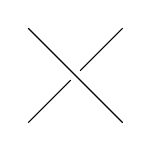
\begin{tikzpicture}[scale=0.6,baseline=-1mm]
	\draw (-1,1) -- (1,-1);
	\draw (-1,-1) -- (-0.1,-0.1);
	\draw (1,1) -- (0.1,0.1);	
\end{tikzpicture}
\equiv
\alpha
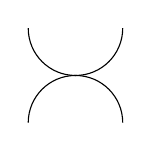
\begin{tikzpicture}[scale=0.6,baseline=-1mm]
	\draw (-.5,1) arc [start angle=-180, end angle=0, radius=1cm];
	\draw (-.5,-1) arc [start angle=180, end angle=0, radius=1cm];
\end{tikzpicture}
+\beta
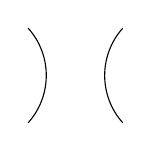
\begin{tikzpicture}[scale=0.6,baseline=-1mm]%\TheAngle grad
	\draw (-1,1) arc [start angle=\TheAngle, end angle=-\TheAngle, radius=1.5cm];
	\draw (1,1) arc [start angle=180-\TheAngle, end angle=180+\TheAngle, radius=1.5cm];
\end{tikzpicture}.
\end{align*}
Its dual has the same diagrams, but both $\alpha$ and $\beta$ are conjugated. It has a very nice symmetry, namely: Rotation by $\pi$ is the identity. A rotation by $90^\circ$ exchanges the coefficients.

We thus only need to calculate one product, $R\cdot R^*$. From this we will get one equation, and, from exchanging $\alpha$ and $\beta$, we will also obtain the second equation.

Using the shorthand notation \textbf{DEFINE THIS} for the calculations, we see 
\begin{align*}
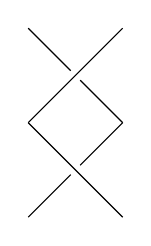
\begin{tikzpicture}[scale=0.6,baseline=5mm]
	\draw (-1,1) -- (1,3);
	\draw (-1,3) -- (-0.1,2.1);
	\draw (1,1) -- (0.1,1.9);	
	\draw (-1,1) -- (1,-1);
	\draw (-1,-1) -- (-0.1,-0.1);
	\draw (1,1) -- (0.1,0.1);
\end{tikzpicture}
= 
\begin{tikzpicture}[scale=0.6,baseline=5mm]
	\begin{scope}
		\coordinate (origin) at (-1.5,3);
			\draw ($(origin) + (-1,1)$) arc [start angle=\TheAngle, end angle=-\TheAngle, radius=1.5cm];
			\draw ($(origin) + (1,1)$) arc [start angle=180-\TheAngle, end angle=180+\TheAngle, radius=1.5cm];
	\end{scope}
	\draw[dotted] (0,4) -- (0,2);
	\begin{scope}	
			\coordinate (origin) at (-1.5,-1);
			\draw ($(origin) + (-1,1)$) arc [start angle=180+\TheAngle, end angle=360-\TheAngle, radius=1.5cm];
			\draw ($(origin) + (-1,-1)$) arc [start angle=180-\TheAngle, end angle=\TheAngle, radius=1.5cm];
	\end{scope}
	%
	\node (circ) at (0,1) {$\circ$};
	%
	\begin{scope}	
			\coordinate (origin) at (1.5,3);
			\draw ($(origin) + (-1,1)$) arc [start angle=180+\TheAngle, end angle=360-\TheAngle, radius=1.5cm];
			\draw ($(origin) + (-1,-1)$) arc [start angle=180-\TheAngle, end angle=\TheAngle, radius=1.5cm];
	\end{scope}
`	\draw[dotted] (0,-2) -- (0,0);
	\begin{scope}
		\coordinate (origin) at (1.5,-1);
			\draw ($(origin) + (-1,1)$) arc [start angle=\TheAngle, end angle=-\TheAngle, radius=1.5cm];
			\draw ($(origin) + (1,1)$) arc [start angle=180-\TheAngle, end angle=180+\TheAngle, radius=1.5cm];
	\end{scope}
\end{tikzpicture}
=\quad
\begin{tikzpicture}[scale=0.6,baseline=5mm]
	\begin{scope}	
			\coordinate (origin) at (-1.7,3);
			\node (d) at ($(origin)+(-1.2,0)$) {$d$};
			\draw ($(origin) + (-1,1)$) arc [start angle=180+\TheAngle, end angle=360-\TheAngle, radius=1.5cm];
			\draw ($(origin) + (-1,-1)$) arc [start angle=180-\TheAngle, end angle=\TheAngle, radius=1.5cm];
	\end{scope}
	\draw[thick] (0,-2) -- (0,4);
		\begin{scope}	
			\coordinate (origin) at (1.5,3);
			\draw ($(origin) + (-1,1)$) arc [start angle=180+\TheAngle, end angle=360-\TheAngle, radius=1.5cm];
			\draw ($(origin) + (-1,-1)$) arc [start angle=180-\TheAngle, end angle=\TheAngle, radius=1.5cm];
	\end{scope}
	\draw[thick] (-3.2,1) -- (3.2,1);
		\begin{scope}	
			\coordinate (origin) at (-1.7,-1);
			\draw ($(origin) + (-1,1)$) arc [start angle=180+\TheAngle, end angle=360-\TheAngle, radius=1.5cm];
			\draw ($(origin) + (-1,-1)$) arc [start angle=180-\TheAngle, end angle=\TheAngle, radius=1.5cm];
	\end{scope}
	\begin{scope}
		\coordinate (origin) at (1.5,-1);
			\draw ($(origin) + (-1,1)$) arc [start angle=\TheAngle, end angle=-\TheAngle, radius=1.5cm];
			\draw ($(origin) + (1,1)$) arc [start angle=180-\TheAngle, end angle=180+\TheAngle, radius=1.5cm];
	\end{scope}
\end{tikzpicture}
\end{align*}
and we thus get two equations that must be satisfied. These are
\begin{align*}
\tag{I}
d\left\vert \alpha \right\vert^2 + [\alpha*\beta] &= 0\\
\tag{II}
d\left\vert \beta \right\vert^2 + [\alpha*\beta] &= 0,
\end{align*}
where $[x*y]\equiv x^*y+y^*x=2\left( \Re{x}\Re{y} + \Im{x}\Im{y} \right)$. 

These equations admit non-trivial solutions. One family of perfect morphisms is for example the one-parameter-family
\begin{align*}
R(a)\equiv
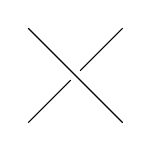
\begin{tikzpicture}[scale=0.6,baseline=-1mm]
	\draw (-1,1) -- (1,-1);
	\draw (-1,-1) -- (-0.1,-0.1);
	\draw (1,1) -- (0.1,0.1);	
\end{tikzpicture}
(a)
\equiv
a\cdot
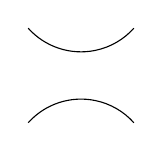
\begin{tikzpicture}[scale=0.6,baseline=-1mm]
	\draw (-1,1) arc [start angle=180+\TheAngle, end angle=360-\TheAngle, radius=1.5cm];
	\draw (-1,-1) arc [start angle=180-\TheAngle, end angle=\TheAngle, radius=1.5cm];
\end{tikzpicture}
-\left( \frac{d}{2} + i\sqrt{1-\frac{d^2}{4}} \right)a\cdot 
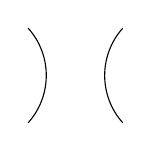
\begin{tikzpicture}[scale=0.6,baseline=-1mm]%\TheAngle grad
	\draw (-1,1) arc [start angle=\TheAngle, end angle=-\TheAngle, radius=1.5cm];
	\draw (1,1) arc [start angle=180-\TheAngle, end angle=180+\TheAngle, radius=1.5cm];
\end{tikzpicture}
\end{align*}
for trivalent categories with loop value $-2 < d < 2$. Indeed,
\begin{align*}
	d\left\vert \alpha \right\vert^2 + [\alpha*\beta] &= da^2 - 2\frac{da^2}{2} = 0
\end{align*}
and
\begin{align*}
d\left\vert \beta \right\vert^2 + [\alpha*\beta] &= d\left( \frac{d^2}{4} +1  - \frac{d^2}{4} \right)a^2 - 2\frac{da^2}{2} =0.
\end{align*}
For $a=\pm 1$, we have $\left\vert \beta \right\vert^2 = 1$, that is $R(\pm 1)\cdot R(\pm 1)^* = \id_2$: Both are isometries.

The defining equations are symmetric with respect to both the exchange of $\alpha$ and $\beta$, and complex conjugation. We can therefore list all 4 solutions that have been found by \texttt{sage} in a concise manner in \ref{table:solutions_r-matrix}.

\begin{table}\centering
	\begin{tabular}[c]{ | c | c | }
		\hline
		$\alpha$ & $\beta$ \\
		\hhline{|=|=|}
		\raisebox{-2.5pt}{$\left(-d \pm i \sqrt{4-d^2}\right) \frac{a}{2}$} & \raisebox{-2.5pt}{$a$}\\[5pt]
		\hline
		\raisebox{-2.5pt}{$a$} & \raisebox{-2.5pt}{$\left(-d \pm i \sqrt{4-d^2}\right) \frac{a}{2}$}\\[5pt]
		\hline
	\end{tabular}
	\caption[Solutions for the generalized $R$-matrix]{Solutions for the generalized $R$-matrix, valid in categories where $\lvert d \rvert < 2$}
	\label{table:solutions_r-matrix}
\end{table}
